\documentclass[a4paper,11pt]{report}
 
% Import des extensions
\usepackage[T1]{fontenc}
\usepackage[utf8]{inputenc}
\usepackage[francais]{babel}
\usepackage{graphicx}
\usepackage{color}
\usepackage{colortbl}
\usepackage{geometry}
\usepackage{hyperref}
\usepackage{fullpage}
\usepackage{eso-pic}
\geometry{hmargin=2.5cm,vmargin=3.5cm}


\newcommand{\blap}[1]{\vbox to 0pt{#1\vss}}
\newcommand\AtUpperLeftCorner[3]{%
\put(\LenToUnit{#1},\LenToUnit{\dimexpr\paperheight-#2}){\blap{#3}}%
}
\newcommand\AtTopCenterPage[2]{%
\put(\LenToUnit{.5\paperwidth},\LenToUnit{\dimexpr\paperheight-#1}){\blap{\hbox to 0pt{\hss#2\hss}}}%
}
\newcommand\AtUpperRightCorner[3]{%
\put(\LenToUnit{\dimexpr\paperwidth-#1},\LenToUnit{\dimexpr\paperheight-#2}){\blap{\llap{#3}}}%
}


\author{Dylan Bideau, Julien Turpin, Pierre Bogrand, Guillaume Vincenti}
\title{\huge{Nautilus - Carnet de Bord}}

\begin{document}
\makeatletter
\begin{titlepage}

	\AddToShipoutPicture{
		\AtUpperLeftCorner{1.5cm}{1cm}{
\includegraphics[width=4cm]{Illustrations/ensea.png}}
	}
	\begin{center}
		\vspace*{10cm}
		\textsc{\@title}
		\vspace*{0.5cm}
		\hrule
		\vspace*{0.5cm}
		\large{\@author}
	\end{center}
	\vspace*{9.2cm}
	\begin{center}
		\large{\@date}
	\end{center}
\end{titlepage}
\ClearShipoutPicture

\renewcommand{\contentsname}{Sommaire}
\tableofcontents


\chapter{Dylan Bideau}
	\section{Configuration Raspberry}
		\subsection{Raspbian}
			Tout d'abord il a fallu installer \underline{Raspbian} sur nos Raspberry Pi. \newline
			Nous l'avons téléchargé ici :\newline
			\url{https://www.raspberrypi.org/downloads/raspbian/}
			\newline Puis grâce à \underline{Win32DiskImager}, nous l'avons installé sur la carte. Ensuite il a fallu trouver un clavier, une souris et un ecran pour pouvoir acceder à notre Raspberry. Pour nos besoin futur il nous faut fixer l'adresse IP de la carte en modifiant \underline{cmdline.txt} sur la base de la microSD de la Raspberry. Nous avons choisit de commencer toutes les notre par 169.254.14. puis 01 pour Julien, 02 pour Pierre et Guillaume et 03 pour Dylan.
			
		\subsection{VNC server}
			\subsubsection{Partie Raspberry}
			Dans un second temps, nous avons voulu interagir avec la Raspberry sans avoir à utiliser un nouvel ecran, 			souris, clavier. Pour cela, nous utilisons VNC pour se connecter à distance avec un cable ethernet. \newline
			Voici le tutoriel dont nous nous sommes inspiré :\newline
			\url{http://www.framboise314.fr/prenez-vraiment-la-main-a-distance-sur-votre-raspberry-pi-avec-x11vnc/}
			\newline Tout d'abord, il faut mettre à jour le systeme :
			\begin{figure}[!h]
				\begin{center}
					
\includegraphics{Illustrations/1.png}
				\end{center}
			\end{figure}
			\newline Puis nous installons VNC sur notre carte :
			\begin{figure}[!h]
				\begin{center}
					
\includegraphics{Illustrations/2.png}
				\end{center}
			\end{figure}
			\newpage L'installation fini, il faut aller dans le menu pour configurer VNC server :
			\begin{figure}[!h]
				\begin{center}
					
\includegraphics[scale=0.5]{Illustrations/3.png}
				\end{center}
			\end{figure}
			\newline Nous allons utilisé le port 5900 pour notre connection à distance
			\begin{figure}[!h]
				\begin{center}
					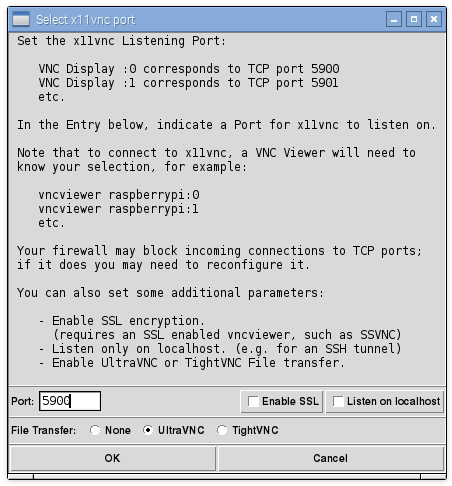
\includegraphics[scale=0.5]{Illustrations/4.png}
				\end{center}
			\end{figure}
			\newline Après avoir appuyé sur OK, nous cochons 3 cases qui nous permettront de nous connecter à distance :
			\begin{figure}[!h]
				\begin{center}
					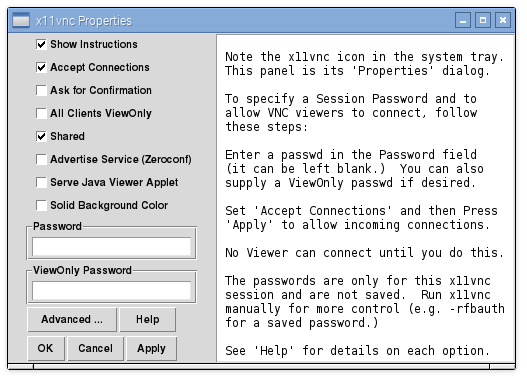
\includegraphics[scale=0.5]{Illustrations/5.png}
				\end{center}
			\end{figure}
			\newline En tant que password, nous avons laisser "raspberry" le code de base de la carte. Le serveur est donc lançé en manuelle.
			\newline \newline Maintenant il nous faut demarrer automatiquement le serveur VNC à chaque demarrage pour ne pas avoir à le lancer manuellement à chaque lancement. Nous allons pour cela crée un fichier mot de passe :
			\begin{figure}[!h]
				\begin{center}
					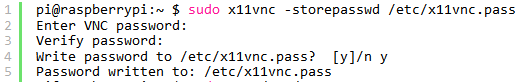
\includegraphics{Illustrations/7.png}
				\end{center}
			\end{figure}
			\newline Pour finir il faut crée le service qui va se lancer à chaque demarrage :
			\begin{figure}[!h]
				\begin{center}
					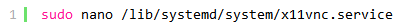
\includegraphics{Illustrations/8.png}
				\end{center}
			\end{figure}
			\newline Et y ecrire cela :
			\begin{figure}[!h]
				\begin{center}
					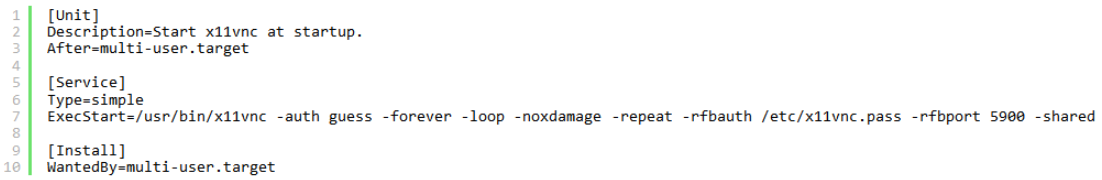
\includegraphics[scale=0.5]{Illustrations/9.png}
				\end{center}
			\end{figure}
			\newline Il reste plus qu'à demander au systeme de le prendre en compte :
			\begin{figure}[!h]
				\begin{center}
					
\includegraphics{Illustrations/10.png}
				\end{center}
			\end{figure}
			\newline Maintenant passons à la partie PC \newpage
			
			\subsubsection{Partie PC}
			Il suffit d'installer VNC viewer sur nos PC, qui se trouve ici :
			\url{https://www.realvnc.com/en/connect/download/viewer/}
			\newline en voici le resultat :
			\begin{figure}[!h]
				\begin{center}
					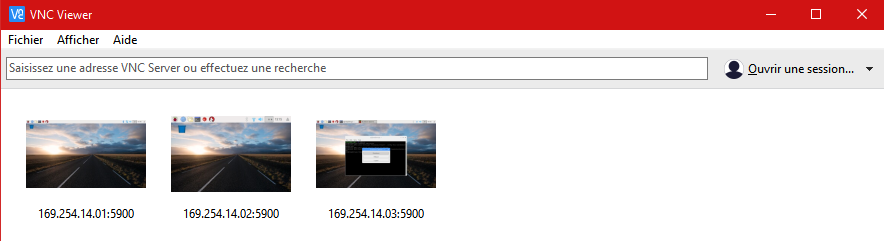
\includegraphics[scale=0.5]{Illustrations/6.png}
				\end{center}
			\end{figure}
			
		\subsection{Les Cameras}
		
		\subsubsection{Camera V2}
		
			Tout d'abord il faut brancher la camera au port prévu sur la raspberry. \newline
			Puis nous devons activer la camera dans les configurations de la rapsberry :
			\begin{figure}[!h]
				\begin{center}
					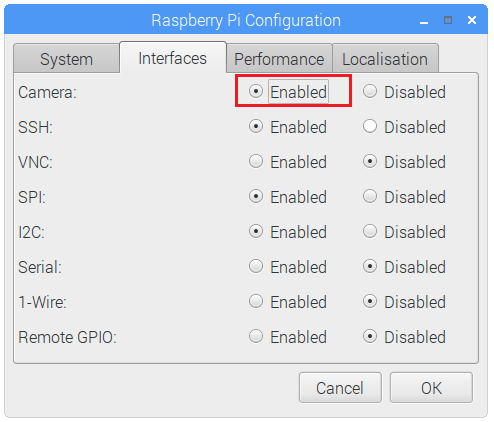
\includegraphics[scale=0.7]{Illustrations/11.png}
				\end{center}
			\end{figure}
		  \newline Nous créeons ensuite le script Python qui va permettre d'envoyer le flux video en streaming sur une IP (169.254.14.0X:8000)
			\begin{figure}[!h]
				\begin{center}
					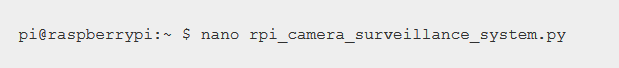
\includegraphics[scale=0.7]{Illustrations/12.png}
				\end{center}
			\end{figure}
			\newline Le code est stocké sur notre gitHub.\newpage
			Puis nous demarrons notre flux IP par cette commande :
			\begin{figure}[!h]
				\begin{center}
					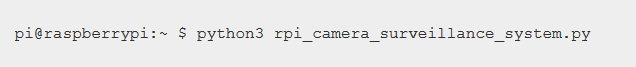
\includegraphics[scale=0.7]{Illustrations/13.png}
				\end{center}
			\end{figure}
			
			\subsubsection{Camera C170 Logitech}
			
			Nous installons Motion, un systeme qui permet de gerer une camera exterieur de façon très personnalisée \newline Tout d'abord installons le :
			\begin{figure}[!h]
				\begin{center}
					
\includegraphics{Illustrations/14.png}
				\end{center}
			\end{figure}
			\newline On va créer un dossier dans lequel les informations et instantanés seront archivées :
			\begin{figure}[!h]
				\begin{center}
					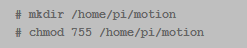
\includegraphics{Illustrations/15.png}
				\end{center}
			\end{figure}
			\newline On va s’intéresser maintenant au fichier de configuration :
			\begin{figure}[!h]
				\begin{center}
					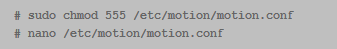
\includegraphics{Illustrations/16.png}
				\end{center}
			\end{figure}
			\newline Le fichier de configuration est sur github.
			\newline Le daemon (service) motion est désactivé par défaut, pour l'autoriser:
			\begin{figure}[!h]
				\begin{center}
					
\includegraphics{Illustrations/17.png}
				\end{center}
			\end{figure}
			
			\chapter{Julien Turpin}

\chapter{Pierre et Guillaume}

\end{document}
